The Raspberry Pi 3 is a single-board computer that accepts MIPI cameras. This device will be used to connect an infrared MIPI Camera and stream a live video fee from the camera via ethernet. In order to avoid connectivity issues with the Jetson TK-1, the Raspberry Pi 3 has been configured with a static IP address. To assure that the live video fee has a small latency, the Raspberry Pi 3 will be connected to a router. The video feed is being streaming using VLC. 

%%%Change Pictures
\begin{figure}[h!]
	\centering
 	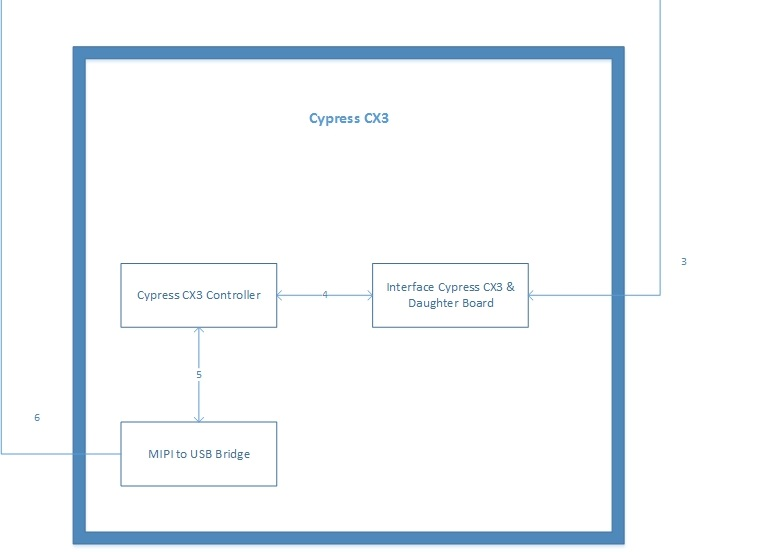
\includegraphics[width=0.60\textwidth]{images/Cypress}
 \caption{Jetson Subsystem Diagram}
\end{figure}


\subsection{Central Processing Unit}
The CPU of the Raspberry Pi is connected to multiple components. One of those components is the camera connector that needs to have a 15 pin ribbon cable in order to accurately receive a video feed from the MIPI camera. In this product, the camera connector is connected to an HDMI Extension Board via a ribbon cable. The CPU of this device also sends the live video fee using VLC via ethernet. All the user needs to have to capture the live video feed is the static IP address of the Raspberry Pi 3. 

%%%Update Imagei
\begin{figure}[h!]
	\centering
 	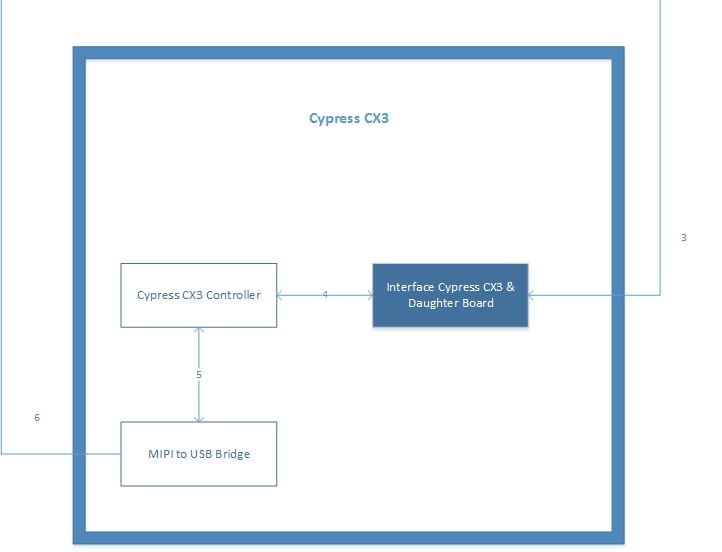
\includegraphics[width=0.60\textwidth]{images/Cypress_Interface}
 \caption{GPID Interface}
\end{figure}

\subsubsection{Assumptions}
The user knows how to connect to the Raspberry Pi 3 via SSH using the Jetson TK-1 terminal.

\subsubsection{Responsibilities}
The responsibility of the Raspberry Pi 3 CPU is to start the live video stream.

\subsubsection{Subsystem Interfaces}

\begin{table}[H]
\caption {Central Processing Unit}
\begin{center}
	\begin{tabular}{ | p{1cm} | p{6cm} | p{3cm} | p{3cm} |}
	\hline
	ID & Description & Inputs & Outputs \\ \hline
	\#01 & HDMI Extension Board & \pbox{3cm}{Input 1 - MIPI Data} & \pbox{3cm}{Output 1 - MIPI Power \\ Output 2 - MIPI Clock} \\ \hline
	\#02 & Ethernet Connector & \pbox{3cm}{Input 1 - RX D2+ \\ Input 2 - RX D2- \\Input 3 - BI D3+ \\ Input 4 - BI D3- \\ Input 5 - BI D4+ \\Input 6 - BI D4-} & \pbox{3cm}{Output 1 - RX D2+ \\ Output 2 - RX D2- \\ Output 3 - BI D3+ \\ Output 4 - BI D3- \\ Output 5 - BI D4+ \\ Output 6 - BI D4-} \\ \hline
	\end{tabular}
\end{center}
\end{table}

\subsection{HDMI Extension Board}
The sole purpose of the HDMI Extension Board is to give the user a longer distance between the MIPI camera and Raspberry Pi 3 in order to make the device more comfortable to the user. The HDMI Extension Board consists of two identical boards that are connected with an HDMI cable. One of the boards is connected via a ribbon cable to the Raspberry Pi 3 while the other board is connected to the Arducam Spy Camera for Raspberry Pi. The HDMI cable is used to send and receive data from and to the Raspberry Pi 3.

%%Update Picture + Caption
\begin{figure}[h!]
	\centering
	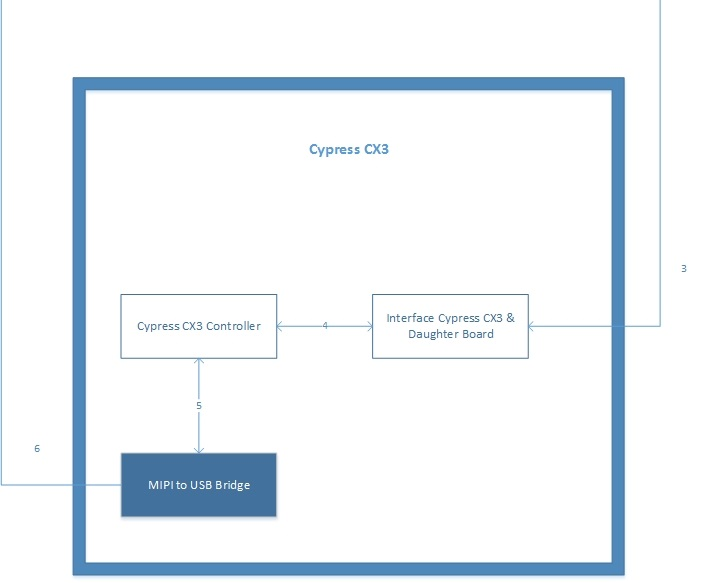
\includegraphics[width=0.60\textwidth]{images/Cypress_MIPI}
	\caption{MIPI to USB Subsystem}
\end{figure}

\subsubsection{Assumptions}
The HDMI cable connected between both boards is fully functional and compatible with both boards.

\subsubsection{Responsibilities}
The HDMI Extension Boards are responsible with interfacing the infrared MIPI camera and the Raspberry Pi 3, and capture and sending a video feed.

\subsubsection{Subsystem Interfaces}
\begin{table}[H]
\caption{HDMI Extension Board}
\begin{center}
	\begin{tabular}{ | p{1cm} | p{6cm} | p{3cm} | p{3cm} |}
	\hline
	ID & Description & Inputs & Outputs \\ \hline
	\#03 & Board Connected To Raspberry Pi 3 & \pbox{3cm}{Input 1 - 3.3V \\ Input 2 - GND \\ Input 3 - LVDS Data 0 to 1 +/- \\ Input 4 - LVDS CLK +/-} & \pbox{3cm}{Output 1 - 3.3V \\ Output 2 - GND \\ Output 3 - LVDS Data 0 to 1 +/- \\ Output 4 - LVDS CLK +/-} \\ \hline
	\#04 & Both HDMI Extension Boards Connected Together & \pbox{3cm}{Input 1 - 3.3V \\ Input 2 - GND \\ Input 3 - LVDS Data 0 to 1 +/- \\ Input 4 - LVDS CLK +/-} & \pbox{3cm}{Output 1 - 3.3V \\ Output 2 - GND \\ Output 3 - LVDS Data 0 to 1 +/- \\ Output 4 - LVDS CLK +/-} \\ \hline
	\#05 & HDMI Extension Board to MIPI Camera & \pbox{3cm}{Input 1 - MIPI Data 0 to 1 +/- \\ Input 2 - MIPI CLK +/-} & \pbox{3cm}{Output 1 - 3.3V \\ Output 2 - GND \\ Output 3 - LVDS Data 0 to 1 +/- \\ Output 4 - LVDS CLK +/-} \\ \hline
	\end{tabular}
\end{center}
\end{table} 


\subsection{CMOS}
The Arducam Sensor Spy Camera for Raspberry Pi has an Omnivision OV5647 sensor in which the CMOS memory chip is used to convert the data collected from the camera into RAW RGB that a computer can use to manipulate the data.

%Update Picture
\begin{figure}[h!]
	\centering
	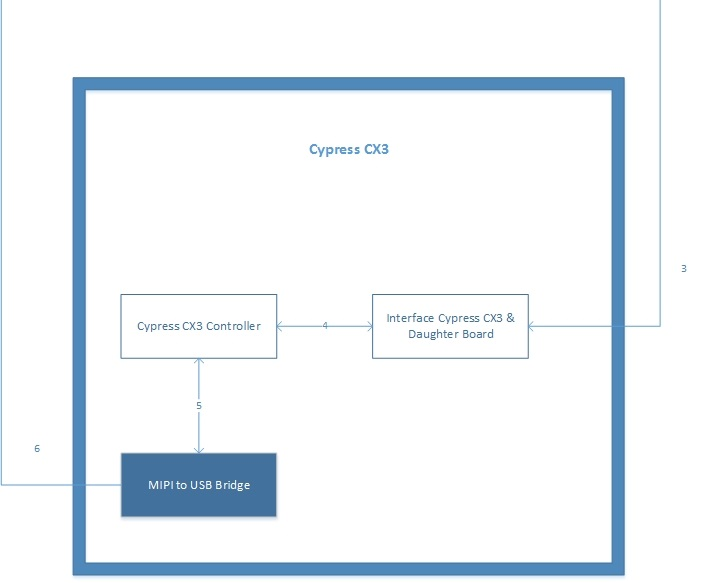
\includegraphics[width=0.60\textwidth]{images/Cypress_MIPI}
	\caption{MIPI to CMOS Conversion \& CMOS-HDMI Data Transfer}
\end{figure} 

\subsubsection{Assumptions}
The CMOS sensor on the MIPI camera is fully functional and has not been damaged during the removal of the infrared filter.

\subsubsection{Responsibilities}
The CMOS sensor converts the images captured from the MIPI camera to a RAW RGB format that can be used by the software to track the user's eye.

\subsubsection{Subsystem Interface}

\begin{table}[H]
\caption{CMOS Sensor OV5647}
\begin{center}
	\begin{tabular}{ | p{1cm} | p{6cm} | p{3cm} | p{3cm} |}
	\hline
	ID & Description & Inputs & Outputs \\ \hline
	\#06 & CMOS to HDMI & \pbox{3cm}{Input 1 - CLK +/-} & \pbox{3cm}{Output 1 - MIPI Data 0 to 1 +/-} \\ \hline
	\#07 & CMOS to MIPI & \pbox{3cm}{Input 1 - MIPI Data 0 to 1 +/-} & \pbox{3cm}{Output - CLK +/-} \\ \hline 
	\end{tabular}
\end{center}
\end{table}

\subsection{MIPI Camera}
The Arducam Sensor Spy Camera for Raspberry Pi is the camera that has been selected to work on this project. Other cameras that are compatible with Raspberry Pi may also work on the eye tracker system. The only modification that needs to be made to this camera is to remove the infrared filter from the camera.

%%%Update Pictures
\begin{figure}[h!]
	\centering
	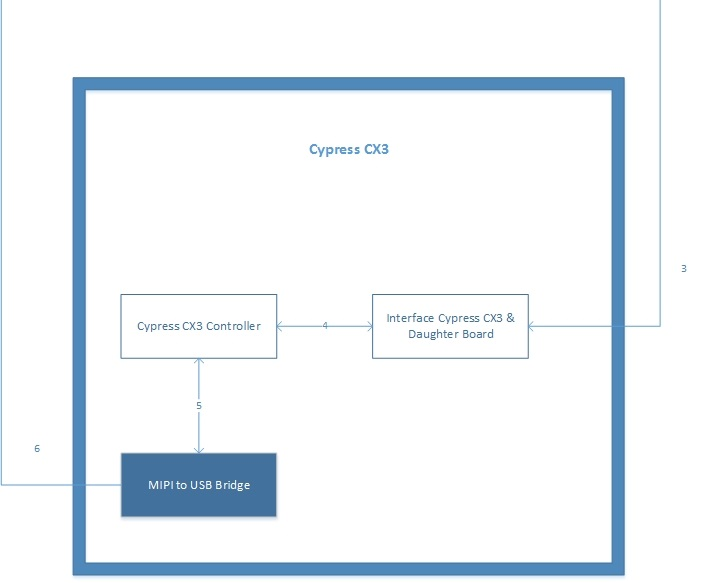
\includegraphics[width=0.60\textwidth]{images/Cypress_MIPI}
	\caption{MIPI to HDMI Connection \& MIPI to CMOS Connection}
\end{figure}

\subsubsection{Assumptions}
The camera used in the project is fully compatible with the Raspberry Pi 3, the camera has not been damaged during the infrared filter removal, and an infrared pass filter has been placed between the lens and the CMOS sensor.

\subsubsection{Responsibilities}
The responsibility of the MIPI Camera is to capture infrared video and send it to the Raspberry Pi in order to stream the video via ethernet.

\begin{table}[H]
\caption{MIPI Infrared Camera}
\begin{center}
	\begin{tabular}{ | p{1cm} | p{6cm} | p{3cm} | p{3cm} |}
	\hline
	ID & Description & Inputs & Outputs \\ \hline
	\#08 & MIPI to HDMI & \pbox{3cm}{Input 1 - 3.3V \\ Input 2 - GND} & \pbox{3cm}{} \\ \hline
	\#09 & MIPI to CMOS & \pbox{3cm}{Input 1 - MIPI Data 0 to 1 +/- \\ Input 2 - MIPI CLK +/-} & \pbox{3cm}{Output 1 - MIPI Data 0 to 1 +/-} \\ \hline
	\end{tabular}
\end{center}
\end{table} 
